\documentclass{article}
\usepackage{tikz, comment}
\usepackage{pifont}
\usepackage{fontspec, pgfplots}
\usetikzlibrary{arrows, decorations.markings, decorations.pathreplacing}
\begin{comment}
:Title: Not defined yet
:Tags: absolute value rules;properties of equality, equation rules;equivalence properties of equality;proper subset;set
:Prob: 0.7697;0.6644;0.5953;0.5738;0.5562
:Author: Prof.Hu Ji-shan, HKUST
:Slug: No name yet

Description Here.........
\end{comment}
\begin{document}\centering 

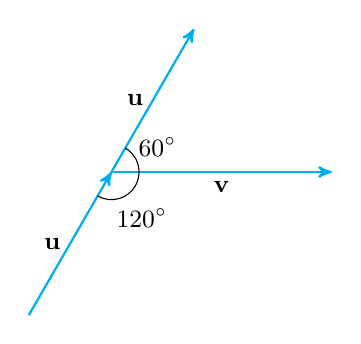
\begin{tikzpicture}[>=latex,xscale=.5*0.35, yscale=.5*0.35][font=\sf\small] 

\draw[cyan, thick, ->, >=stealth'] (0,0)--(16, 0)
node[black, below, midway, pos=0.5, xshift=0, yshift=0, scale=1]{${\bf v}$};

\draw[cyan, thick, ->, >=stealth'] (0,0)--({12*cos(60)}, {12*sin(60)})
node[black, left, midway, pos=0.5, xshift=0, yshift=0, scale=1]{${\bf u}$};

\draw[cyan, thick, <-, >=stealth'] (0,0)--({12*cos(-120)}, {12*sin(-120)})
node[black, left, midway, pos=0.5, xshift=0, yshift=0, scale=1]{${\bf u}$};

\draw[samples=100, smooth, domain=0:60, variable=\x] 
		plot ({2*cos(\x)}, {2*sin(\x)}); 
\node[black, xshift=8, yshift=4, scale=1] at ({2*cos(30)}, {2*sin(30)}) {$60^\circ$};

\draw[samples=100, smooth, domain=0:-120, variable=\x] 
		plot ({2*cos(\x)}, {2*sin(\x)}); 
\node[black, xshift=6, yshift=-8, scale=1] at ({2*cos(-60)}, {2*sin(-60)}) {$120^\circ$};
		
\end{tikzpicture}
\end{document}